\lecture{8. I Will Make a New Covenant}{08}

%------------------------------------------------------------------------------
\section{Introduction}
% this to put in this one:
% There is NO separation between church and personal life.
%--------------------------------------
\begin{frame}
\begin{center}
	
\includegraphics[width=\textwidth]{figures/hopelessness.jpg}
\end{center}

\note{09:30}
\note[item]{In previous lessons we've learned that God wants a relationship with people}
\note[item]{At earlier times He chose a people, the Israelites, and made a special covenant with them.}
\note[item]{Israel rejected this covenant.}
\note[item]{They faced horrible physical and spiritual consequences.}
\note[item]{It's terrifying to think that we, too, may fall under the same judgment of God.}
\note[item]{We might feel a bit like this picture.}
\note[item]{'what must we do to be saved?'}
\note[item]{Today we'll start talking about God's solution for us, the New Covenant.}
\end{frame}

%--------------------------------------
\begin{frame}{God wants a relationship with people}
\framesubtitle{Jeremiah 31:31-34}
	\keyversehiglight{I will make a new covenant}
	
\note{09:32}
\note[item]{Our text text for the class is a prophecy of what this New Covenant will be.}
\note[item]{It's God's solution to bringing a sinful people back into a relationship with Him.}  
\end{frame}

%--------------------------------------
\begin{goals}
\goal Understand what the New Covenant is
\goal Examine why the New Covenant was needed
\goal Assess how God's relationship with His people changed from the Old to the New Covenants

\note{09:34}
\note[item]{We'll look at 5 scriptures and think about what the New Covenants is, why it was needed, and how our relationship with God improved from the Old to the New}
\note[item]{The scriptures are Luke 22:14-23, Eph. 2, Rom. 11:25-32, Heb 10:1-18, and II Cor. 3:7-18}
\note[item]{The flow will be a little different than normal in that we'll revisit each scripture multiple times.}
\note[item]{We'll consider each scripture (most of the scriptures) in the context of the goals.}
\end{goals}

%------------------------------------------------------------------------------
\section{What is the New Covenant?}

%--------------------------------------
\begin{frame}{The New Covenant vs. the Old}
\framesubtitle{Jer. 31:31-34}

\begin{description}[from the least to the greatest]
\item[I will put my law within them] genuine obedience
\item[I will write it on their hearts] inward commitment
\item[I will be their God] a new focus
\item[they shall be my people] it's no longer physical Israel
\item[\ldots they shall all know me] faith not genealogy
\item[from the least to the greatest] there's no distinctions
\item[I will forgive their iniquities] more than overlooking sins
\end{description}

\note{09:36}
\note[item]{A prep for the last 5 lessons.}
\note[item]{law within them -- Christians focus on commitment from the heart not outward rituals (\emph{e.g.}, Pharisees,`whitewashed tombs')}
\note[item]{write it on hearts -- not tablets.  Israelites should have done this (law `when you rise up and lay down').  Christians will get it right.}
\note[item]{I will be their God -- Christians are God's new focus}
\note[item]{They shall be my people -- no longer physical Israel}
\note[item]{\ldots they shall all know me -- from 'no longer teach\ldots' forward says you don't have to teach a Christian how to be saved.  All Christians already `know' God. Not true in the OT. You could be born an Israelite but grow up not knowing the Lord.}
\note[item]{least to greatest -- no distinction between clergy/laity, Jews/gentiles, rich/poor, etc.  In God's kingdom we're all priests.}
\note[item]{forgive their iniquity -- You'll need a better sacrifice for this.}
\end{frame}

%--------------------------------------
\begin{frame}{The New Covenant according to Jesus}
\framesubtitle{Luke 22:14-23}

\begin{columns}[c]
\begin{column}{0.4\textwidth}
	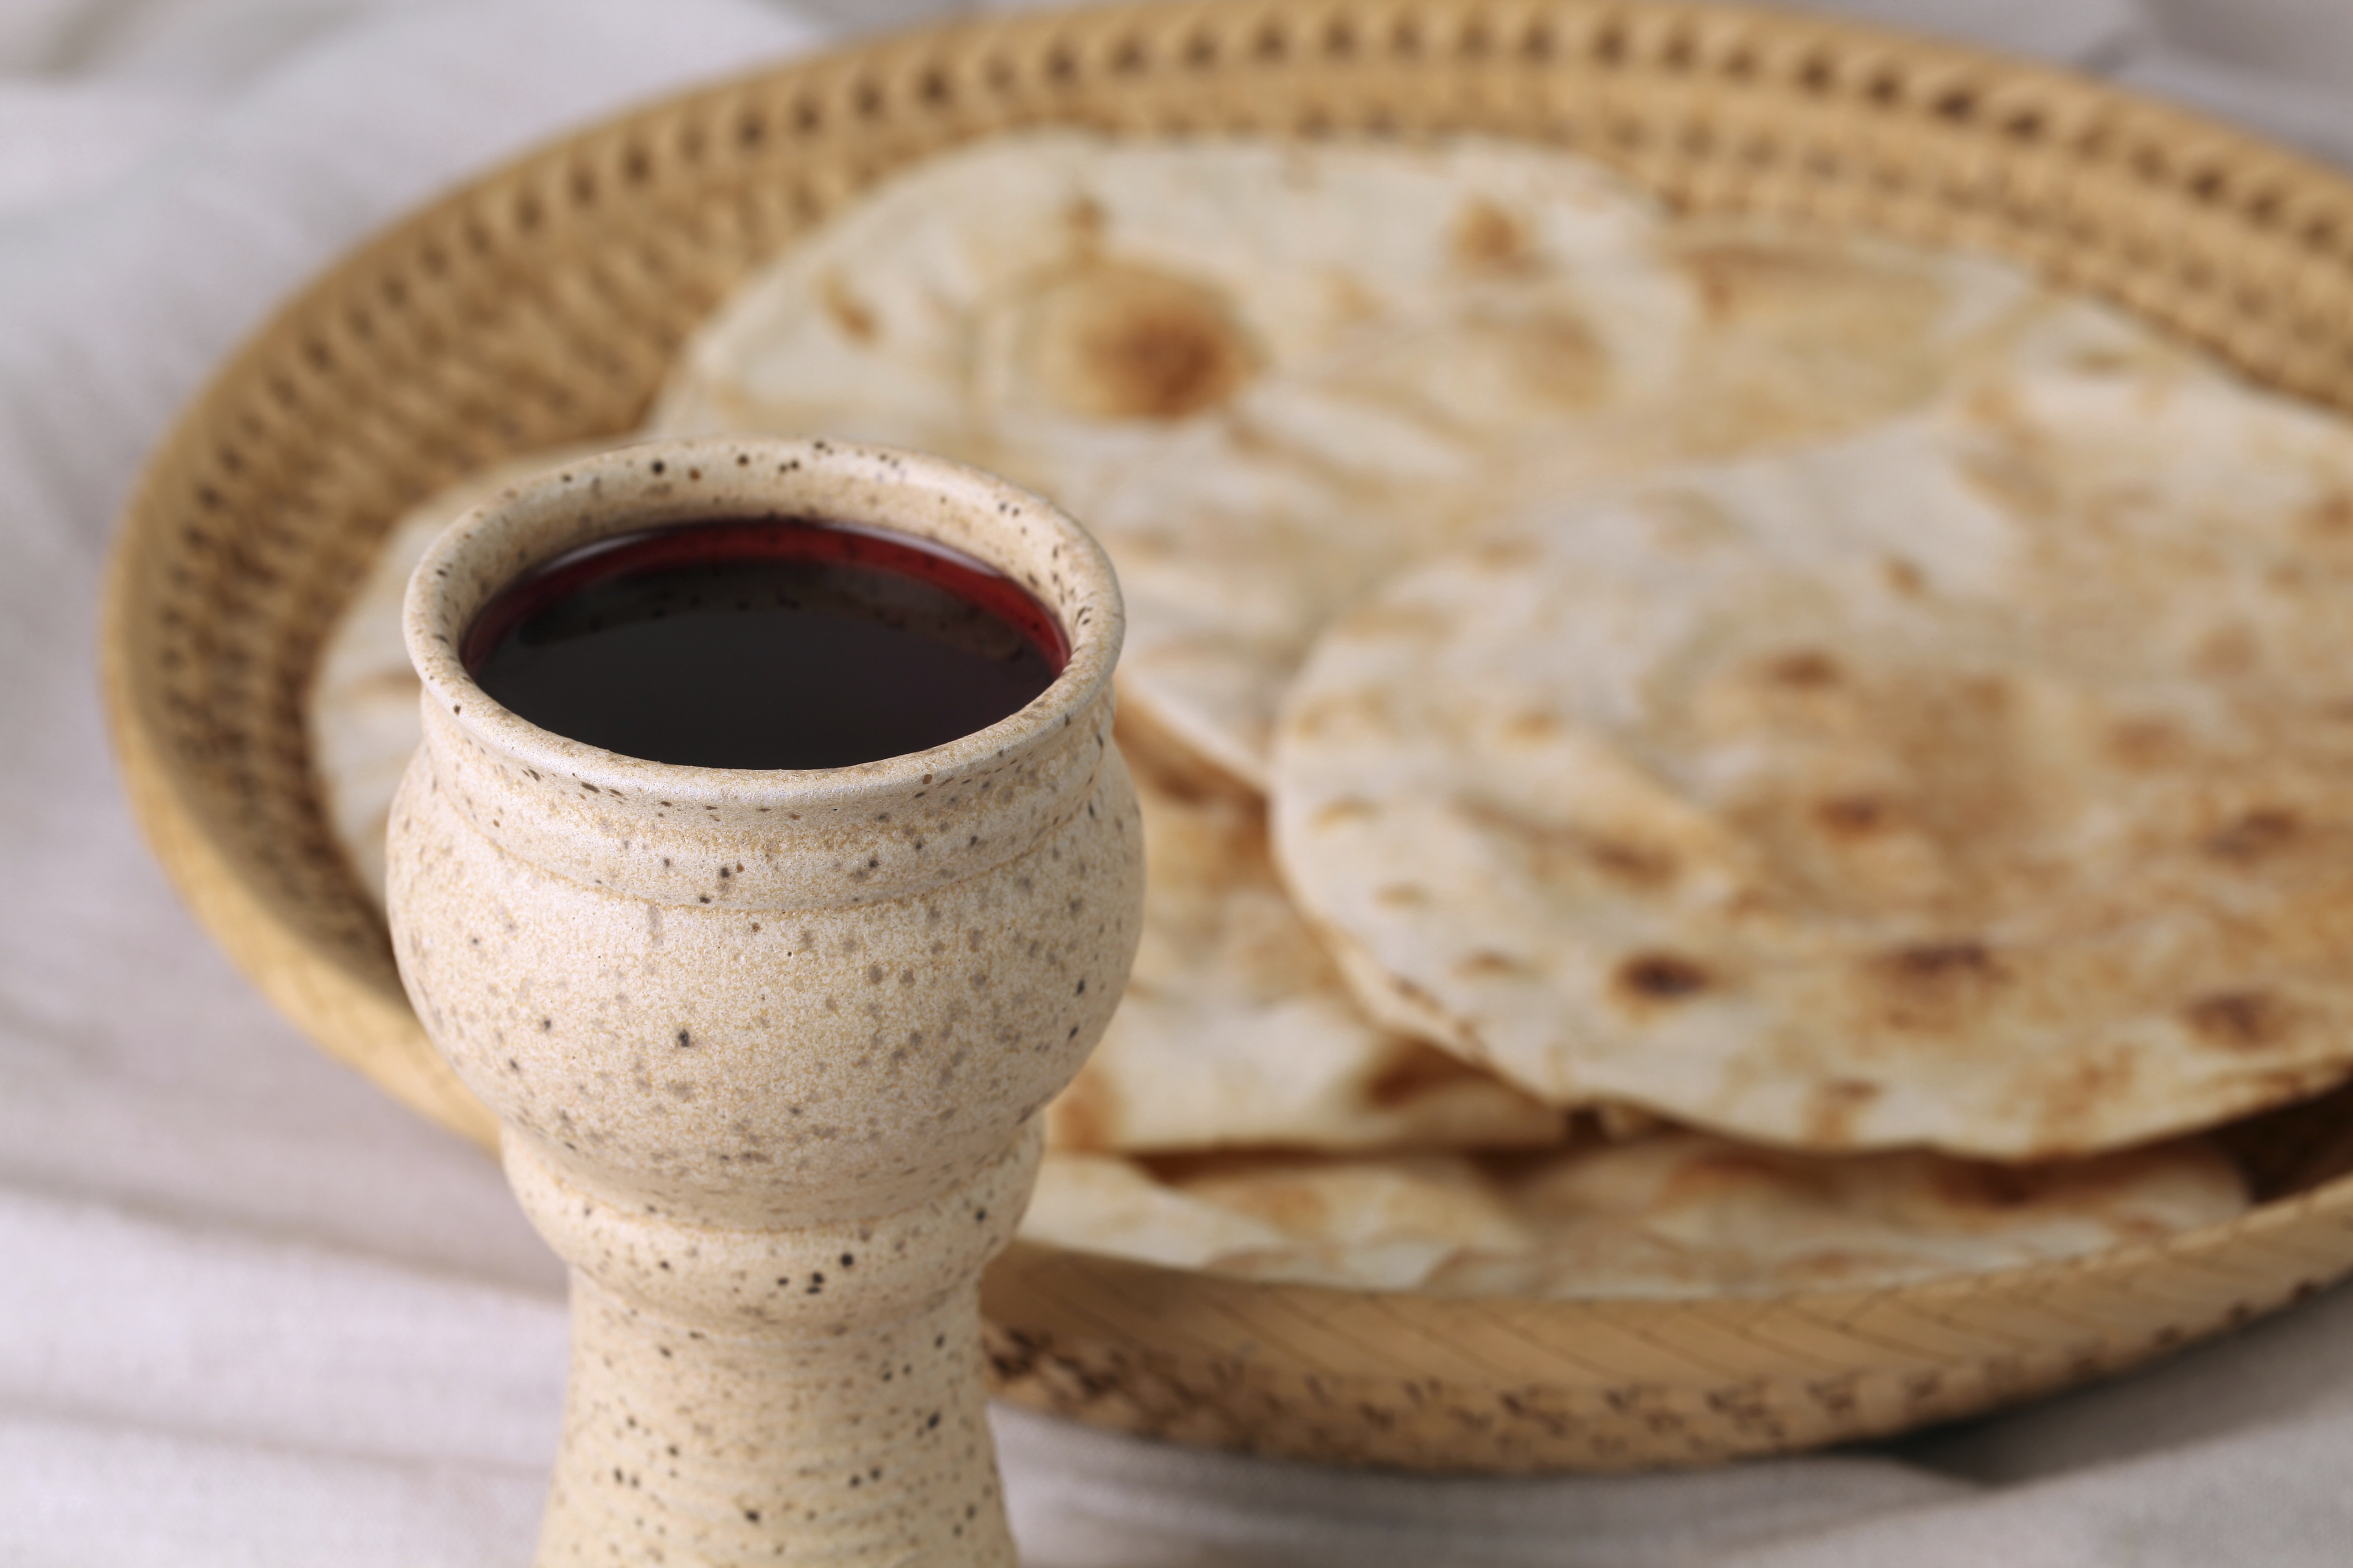
\includegraphics[width=\columnwidth]{figures/communion.jpg}
\end{column}
\begin{column}{0.6\textwidth}
	\begin{itemize}
		\item New Covenant = Kingdom of God
		\item Payment made with Jesus' body.
		\item Signed with Jesus' blood
	\end{itemize}
\end{column}
\end{columns}

\note{09:41}
\note[item]{Jesus talks about the kingdom and the new covenant in the same context.  They are synonyms.}
\note[item]{Two parts of a contract are mentioned here.}
\note[item]{The first is payment for services rendered.}
\note[item]{Note the Jesus says that \emph{he} is paying for \emph{our} side of the contract.}
\note[item]{Second, there's a signature, which really is ratification of the contract.}
\note[item]{When Jesus dies the New Covenant is ratified.}
\note[item]{\emph{If someone says ratification is Pentecost, then I'd say Pentecost is the date of effect.  It's ratified before, but the start date is 50 days later. But, we'll not take the analogy too far.}}
\end{frame}

%--------------------------------------
\begin{frame}{The New Covenant according to Ephesians}
\framesubtitle{Eph. 2}

\begin{columns}[c]
\begin{column}{0.5\textwidth}
	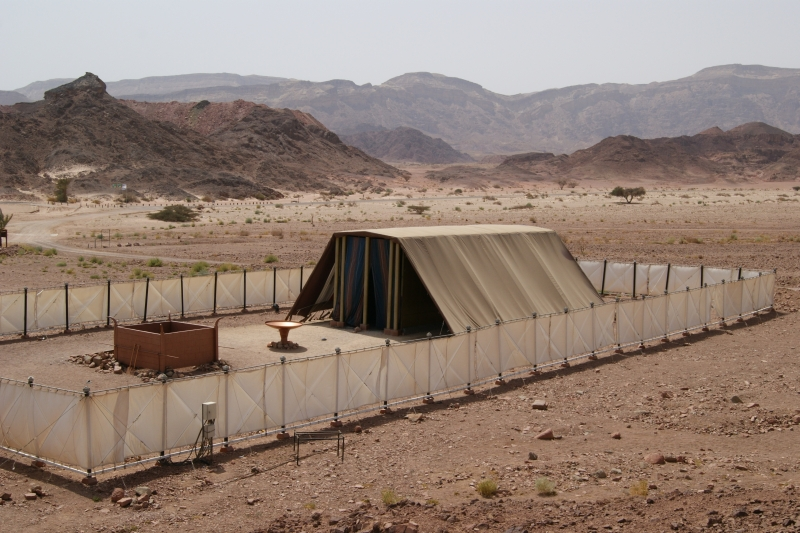
\includegraphics[width=\columnwidth]{figures/tabernacle.jpg}
\end{column}
\begin{column}{0.5\textwidth}
	\begin{itemize}
		\item Life with the Messiah (1-4)
		\item Salvation by grace through faith (5-10)
		\item The end of the Old Covenant (15)
		\item God's Holy Sanctuary (19-21)
	\end{itemize}
\end{column}
\end{columns}

\note{09:43}
\note[item]{New Covenant people will be `resurrected', in more ways than one.}
\note[item]{The end of the Old Covenant - New Covenant is not based on law}
\note[item]{There's no room for boasting since it's not of works}
\note[item]{Holy Sanctuary - Both house (v 19) and tabernacle (v 21)}
\note[item]{Jesus is the cornerstone}
\note[item]{Apostles and prophets build on it}
\note[item]{That house was put together by God and is always growing}
\end{frame}

%--------------------------------------
\begin{frame}{The New Covenant according to Hebrews}
\framesubtitle{Heb. 10}

\begin{columns}[c]
\begin{column}{0.5\textwidth}
	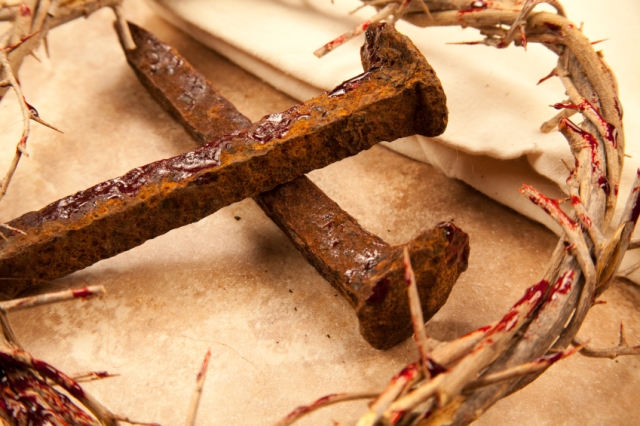
\includegraphics[width=\columnwidth]{figures/jesusSacrifice.jpg}
\end{column}
\begin{column}{0.5\textwidth}
	\begin{itemize}
		\item Jesus' sacrifice is once for all (10)
		\item Jesus' sacrifice sanctifies forever (12)
		\item Jesus' enemies not punished\ldots\emph{yet} (13)
	\end{itemize}
\end{column}
\end{columns}

\note{09:47}
\note[item]{There's only going to be one sacrifice in the New Covenant.}
\note[item]{That sacrifice is going to work for everyone for all time.}
\note[item]{There are pieces of the New Covenant that have yet to be fulfilled}
\note[item]{For instance, judging of the wicked, who by their actions reject the sacrifice of Jesus.}
\end{frame}

%--------------------------------------
\begin{frame}{The New Covenant according to II Corinthians}
\framesubtitle{II Cor. 3:7-18}

\begin{columns}[c]
\begin{column}{0.6\textwidth}
	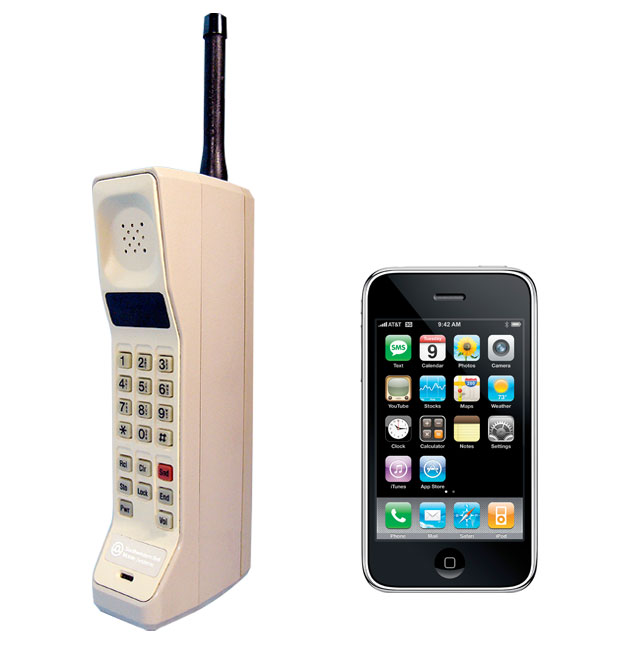
\includegraphics[width=\columnwidth]{figures/oldNewCellphone.jpg}
\end{column}
\begin{column}{0.4\textwidth}
The New Covenant is more glorious than the Old.
\end{column}
\end{columns}

\note{09:50}
\note[item]{Neil already went over this, so we'll just review}
\note[item]{The New Covenant is more glorious}
\note[item]{What does it mean to be more glorious?}
\note[item]{Better.  But, that sort of falls short.}
\note[item]{Here's the best illustration I can come up with.}
\note[item]{Could you image trying to go back and use the cell phone on the left?}
\note[item]{Can you imagine what your 1980's self would think if you went back in time and handed him an iPhone?}
\note[item]{That's a level of improvement that we can comprehend.  The improvement from the Old to the New covenants is much bigger than that.}
\end{frame}
%------------------------------------------------------------------------------
\section{It was needed because\ldots}

%--------------------------------------
\begin{frame}{We were dead with no chance for life}
\framesubtitle{Eph 2.}

\begin{columns}[c]
\begin{column}{0.5\textwidth}
	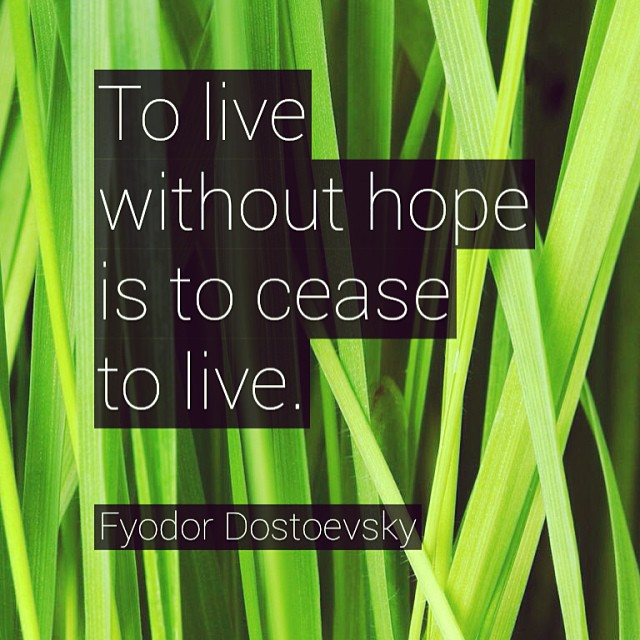
\includegraphics[width=\columnwidth]{figures/withoutHopeQuote.jpg}
\end{column}
\begin{column}{0.5\textwidth}
	\begin{itemize}
		\item We were dead in sins (1-9)
		\item We are Gentiles in the flesh(11-21)
	\end{itemize}
\end{column}
\end{columns}

\note{09:52}
\note[item]{We needed the new covenant because without it we're dead, both physically and spiritually}
\note[item]{We're Gentiles: Excluded from citizenship of Israel, Foreigners to the covenant of promise, Without Hope, Without God}
\note[item]{Does this mean \emph{no} Gentiles were saved in the OT? \emph{Of course not, (e.g. Ruth), but the plan certainly didn't focus on salvation for the whole world.}}

\end{frame}

%--------------------------------------
\begin{frame}{Animal sacrifices are insufficient}
\framesubtitle{Heb. 10:1-18}

\begin{columns}[c]
\begin{column}{0.5\textwidth}
	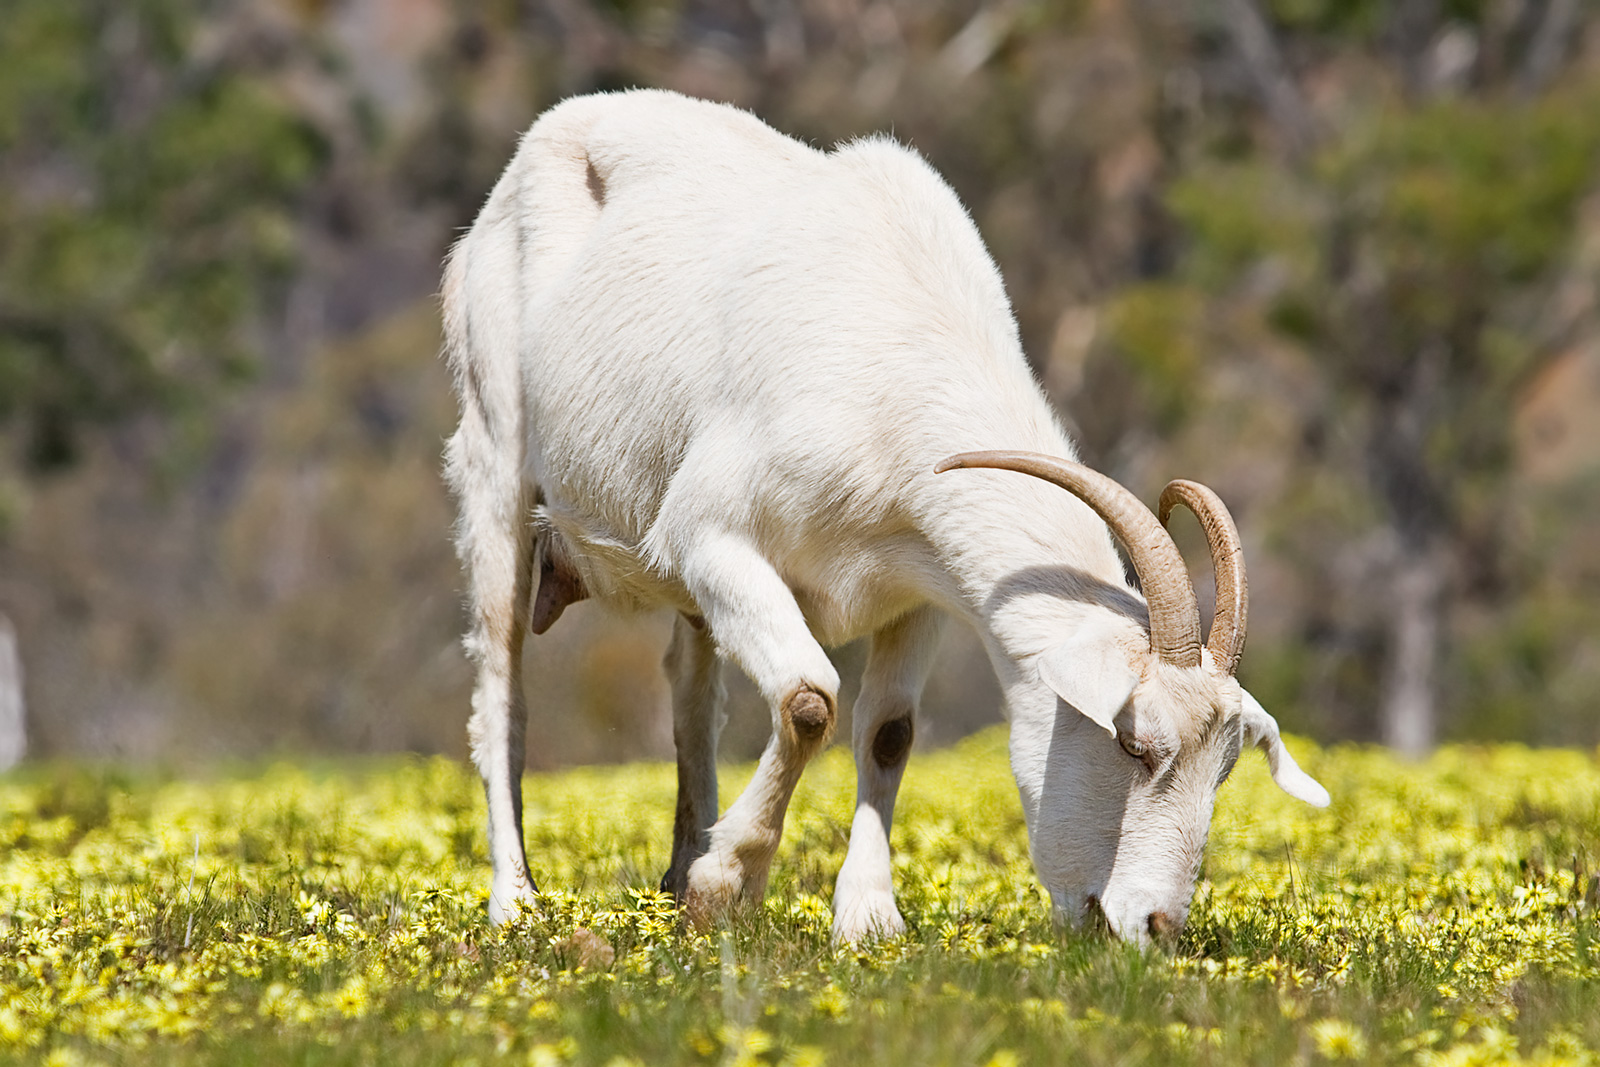
\includegraphics[width=\columnwidth]{figures/goat.jpg}
\end{column}
\begin{column}{0.5\textwidth}
	\begin{itemize}
		\item The Law cannot perfect the worshipers (1-2)
		\item The sacrifices can't really take away sins (3-4)
		\item God doesn't really want animal sacrifice and offering\ldots 
		\item He wants a human offering (5-7)
	\end{itemize}
\end{column}
\end{columns}

\note{09:55}
\note[item]{The argument is that if the sacrifices take away sins, then you don't have to keep offering them.}
\note[item]{How were the sacrifices a `reminder of sin'?  \emph{Well, you had to do it frequently.  It cost you something.  And, you had to be there when the animal was killed.}}

\end{frame}

%--------------------------------------
\begin{frame}{All Israel needs to be saved}
\framesubtitle{Romans 11:25-32}

\begin{columns}[c]
\begin{column}{0.5\textwidth}
	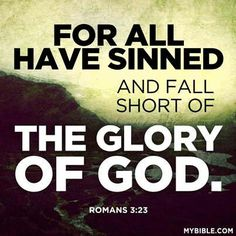
\includegraphics[width=\columnwidth]{figures/forAllHaveSinned.jpg}
\end{column}
\begin{column}{0.5\textwidth}
	\begin{itemize}
		\item Everyone had to be consigned to disobedience
		\item So, a partial hardening came on Israel
		\item Until the Gentiles came in
		\item Christians are now the\\new Israel
	\end{itemize}
\end{column}
\end{columns}

\note{09:55}
\note[item]{Paul makes the same point in chapters 1-3 culminating in v23 `for all have sinned and fall short of the glory of God'}
\note[item]{The hardening of Israel served to bring the Gentiles in by\ldots}
\note[item]{Killing Jesus}
\note[item]{Persecuting the church so that the gospel spread to all places}
\note[item]{There's nothing to suggest all physical Israel would be saved eventually (in a millennial kingdom)}
\note[item]{Paul already said that Israel in the New Covenant is spiritual Rom. 9:6-7}
\end{frame}

%------------------------------------------------------------------------------
\section{A Change in Relationship}

%--------------------------------------
\begin{frame}{We've been brought near to God}
\framesubtitle{Eph 2}

\begin{columns}[c]
\begin{column}{0.4\textwidth}
	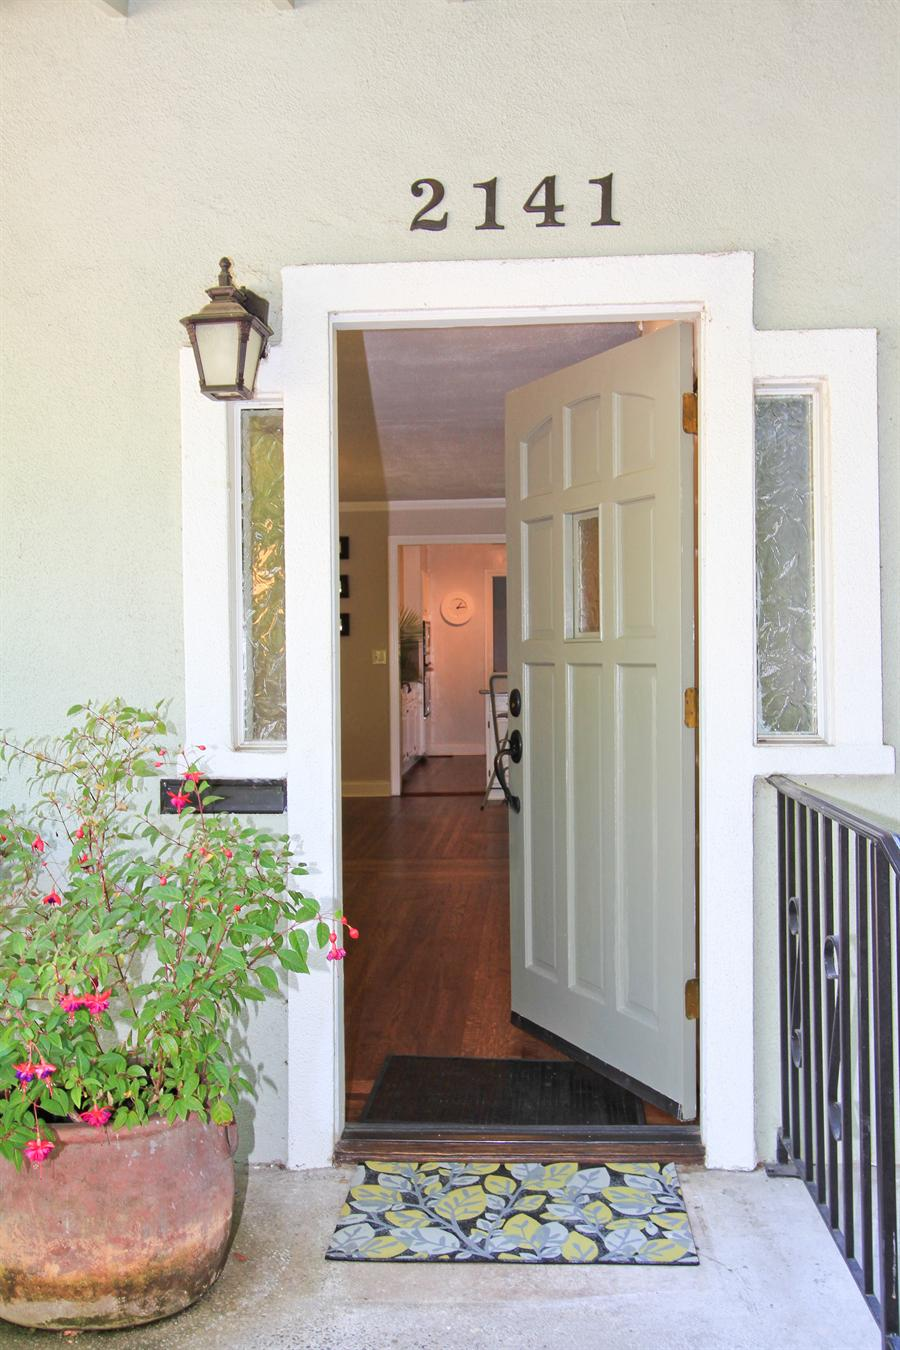
\includegraphics[width=\columnwidth]{figures/openDoor.jpg}
\end{column}
\begin{column}{0.6\textwidth}
	\begin{itemize}
		\item A seat in the heavens (6)
		\item Access to the Father (18)
		\item A member of God's household (19)
	\end{itemize}
\end{column}
\end{columns}

\note{9:58}
\note[item]{Paul makes the same point in chapters 1-3 culminating in v23 `for all have sinned and fall short of the glory of God'}
\note[item]{The hardening of Israel served to bring the Gentiles in by\ldots}
\note[item]{Killing Jesus}
\note[item]{Persecuting the church so that the gospel spread to all places}
\note[item]{There's nothing to suggest all physical Israel would be saved eventually (in a millennial kingdom)}
\note[item]{Paul already said that Israel in the New Covenant is spiritual Rom. 9:6-7}
\end{frame}

%--------------------------------------
\begin{frame}{We've been perfected}
\framesubtitle{Heb. 10:1-18}

\begin{columns}[c]
\begin{column}{0.5\textwidth}
	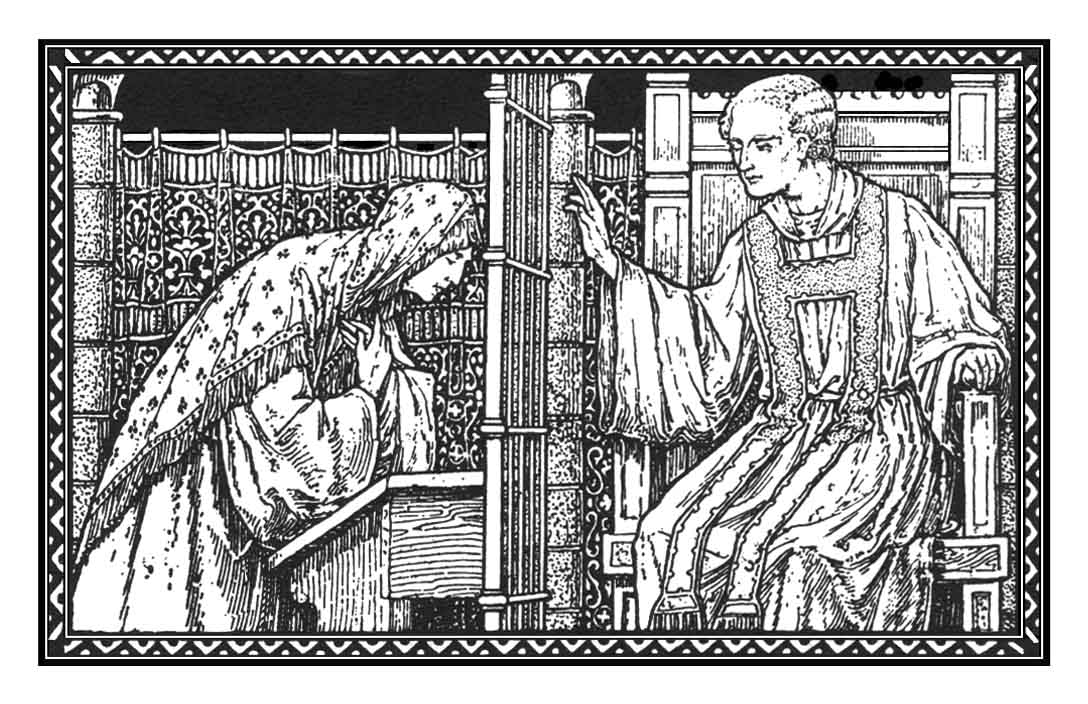
\includegraphics[width=\columnwidth]{figures/penance.jpg}
\end{column}
\begin{column}{0.5\textwidth}
	\begin{itemize}
		\item Jesus has sat down at the right hand of God
		\item He's perfected forevermore those who are sanctified
		\item No longer a need for an offering
	\end{itemize}
\end{column}
\end{columns}

\note{10:01}
\note[item]{Jesus new position suggests that he has completed his earthly work}
\note[item]{Jesus has received His reward and gives us hope that \emph{we} will receive our reward.}
\note[item]{His sacrifice is still sufficient today.}
\note[item]{Think about the effectiveness of Jesus' sacrifice in the context of the catholic practice of penance (picture).}
\note[item]{Penance is basically punishing yourself for sins you committed and has to be done over again when you commit another sin.}
\note[item]{The Hebrew writer would reject such practices on the basis that Jesus' sacrifice is sufficient for the sins you have committed in the past, \emph{and} the sins you will commit in the future.}
\note[item]{Don't continue to beat yourself up over past sins.}
\note[item]{And, don't fret over the `cursing as I die in a car crash' conundrum of unconfessed sin.}
\end{frame}

%--------------------------------------
\begin{frame}{God can have mercy on all}
\framesubtitle{Rom 11:32}

\begin{center}

\includegraphics[height=0.8\textheight]{figures/ladyJustice.jpg}
\end{center}

\note{10:05}
\note[item]{This depiction of lady justice illustrates a few things we'd like to avoid when it comes to our spiritual life.}
\note[item]{The balance: What you've done will be weighed exactly against the standard.}
\note[item]{The blindfold: You can't get out of it because you're special.}
\note[item]{The sword: If the balance finds you guilty, consequences will follow.}
\note[item]{But, God arranged His plan specifically so He could show mercy}
\note[item]{It's hard for us to understand, because we're used to how our justice system works.}
\note[item]{Governments seek out the wrong-doers for the expressed purpose of bringing them to justice.}
\note[item]{Our Lord sought out wrong-doers to help them avoid the justice they deserve.}
\end{frame}

%--------------------------------------
\begin{frame}{We've been set free}
\framesubtitle{II Cor. 3:7-18}


\includegraphics[width=\textwidth]{figures/freedom.jpg}

\note{10:08}
\note[item]{More review from Neil's class.}
\note[item]{What does it freedom \emph{feel} like?}
\note[item]{\emph{Relief}}
\note[item]{\emph{Taking a weight off our shoulders.}}
\note[item]{\emph{Peace}}
\end{frame}

%------------------------------------------------------------------------------
\section{Review}

\begin{frame}{I will make a new covenant}
	\begin{itemize}
		\item The New Covenant is\ldots
		\begin{itemize}
			\item salvation by grace through faith
			\item the forgiveness of sins
			\item the kingdom
			\item paid for by Jesus' sacrifice once for all
			\item the end of the Old Covenant
		\end{itemize}
		\item The New Covenant was needed because\ldots
		\begin{itemize}
			\item we were all dead in sin.
			\item we were Gentiles without hope.
			\item animal sacrifices were insufficient
		\end{itemize}
		\item The New Covenant changed things by\dots
		\begin{itemize}
			\item bringing mercy for all
			\item making us members of God's house
			\item perfecting us forever
		\end{itemize}
	\end{itemize}
	
\note{10:10}
\note[item]{Just go over these and leave time for other to make comments.}
\end{frame}

